%%%%%%%%%%%%%%%%%%%%%%%%%%%%%%%%%%%%%%%%%%%%%%%%%%%%%%%%
%%
\clearpage
\newpage
\section{The cal\_CCF recipe}
\label{ch:the_recipes:cal_CCF_E2DS_spirou}
%%
%%%%%%%%%%%%%%%%%%%%%%%%%%%%%%%%%%%%%%%%%%%%%%%%%%%%%%%%

Computes the CCF for a specific file using a CCF mask, target RV, CCF width and CCF step.

% -------------------------------------------------------
\subsection{The inputs}
% -------------------------------------------------------
The input of \calCCF is as follows:
\begin{cmdbox}
cal_CCF_E2DS_spirou.py night_repository e2dsfile mask rv width step
\end{cmdbox}
\noindent for example
\begin{cmdbox}[title={example}]
cal_CCF_E2DS_spirou.py 20170710 fp_fp02a203_e2ds_AB.fits UrNe.mas 0 10 0.1
\end{cmdbox}
\noindent or
\begin{pythonbox}
import cal_CCF_E2DS_spirou
filename = 'fp_fp02a203_e2ds_AB.fits'
ccf_mask = 'UrNe.mas'
target_rv = 0.0
ccf_width = 10
ccf_step = 0.1
cal_CCF_E2DS_spirou.main(night_repository, filename=e2dsfile, mask=ccfmask, 
                         rv=target_rv, width=ccf_width, step=ccf_step)
\end{pythonbox}

\noindent where:
\begin{itemize}
\item `night\_repository' defines \argnightname
\item `e2dsfile' is the E2DS file to calculate the CCF for
\item `mask' is the name (or full path) of the CCF mask file.

\DevNote{If the CCF mask is not defined as a `full system path' and cannot be found in the current working directory the recipe will search for it in the \definevariable{text:cdata_folder}{const\_data\_folder} (defined in \spirouConst). If it is still not located an error will be raised and the recipe will exit. Therefore in most cases the CCF masks should be located in the \definevariable{text:cdata_folder}{const\_data\_folder} directory.}

\item `rv' is the target radial velocity (central velocity) in km/s
\item `width' is the CCF width (half range in velocity) in km/s
\item `step' is the CCF step in km/s
\end{itemize}

\noindent Filename suffixes allowed are:
\begin{itemize}
	\item *e2ds\_\{fiber\}.fits
\end{itemize}
\noindent where \{fiber\} is the fiber type (i.e. `AB', `A', `B' or `C').

% -------------------------------------------------------
\subsection{The outputs}
% -------------------------------------------------------
The outputs of \calCCF are as follows:

\begin{itemize}

\item \definevariable{text:corfile}{corfile} in form:
\begin{tcustomdir}
\{\reduceddir\}/\{date prefix\}\_\{file\}\_ccf\_\{ccf\_mask\}.fits
\end{tcustomdir}

\item \definevariable{text:ccf_table_file}{ccf\_table\_file} in form:
\begin{tcustomdir}
\{\reduceddir\}/\{date prefix\}\_\{file\}\_ccf\_\{ccf\_mask\}.tbl
\end{tcustomdir}

\end{itemize}


\noindent where `date prefix' is constructed from \argnightname , the file name the `e2dsfile', and \{ccf\_mask\} is `mask' from the inputs.


\noindent for example for \reduceddir\lstinline[style=pythoninline]|='/drs/data/reduced/20170710'|, \lstinline[style=pythoninline]|e2dsfile=fp_fp02a203_e2ds_AB.fits|, and \lstinline[style=pythoninline]|"UrNe.mas"| the output files would be:
\begin{tcustomdir}
\begin{itemize}
\item \path{/drs/data/reduced/20170710/fp_fp02a203_ccf_UrNe_AB.fits}
\item \path{/drs/data/reduced/20170710/fp_fp02a203_ccf_UrNe_AB.tbl}
\end{itemize}
\end{tcustomdir}

% -------------------------------------------------------
\subsection{Summary of procedure}
% -------------------------------------------------------
\begin{enumerate}
\item reads the E2DS file
\item reads the wavelength solution and the flat file
\item corrects for the flat
\item computes photon noise uncertainty
\item gets the CCF mask
\item calculates the CCF for each order
\item fits the CCF for each each
\item averages the CCFs over all orders
\item fits the average CCF over all orders
\item archives the ccf to .fits and .tbl format
\end{enumerate}
\DevNote{Blaze and Flat are currently set to arrays of one. There for no flat or blaze correction is currently done. Blaze file is currently not read and will need to be read to correct for it.}


% -------------------------------------------------------
\newpage
\subsection{Example working run}
% -------------------------------------------------------

An example run where everything worked is below:

\begin{cmdbox}[title={example}]
cal_CCF_E2DS_spirou.py 20170710 fp_fp02a203_e2ds_AB.fits UrNe.mas 0 10 0.1
\end{cmdbox}
\begin{cmdboxprintspecial}[fontupper=\tiny, fontlower=\tiny]
@gHH:MM:SS.S -   || *****************************************@g
@gHH:MM:SS.S -   || * SPIROU \@(#) Geneva Observatory (VERSION)@g
@gHH:MM:SS.S -   || *****************************************@g
@gHH:MM:SS.S -   ||(dir_data_raw)      DRS_DATA_RAW=/drs/data/raw@g
@gHH:MM:SS.S -   ||(dir_data_reduc)    DRS_DATA_REDUC=/drs/data/reduced@g
@gHH:MM:SS.S -   ||(dir_calib_db)      DRS_CALIB_DB=/drs/data/calibDB@g
@gHH:MM:SS.S -   ||(dir_data_msg)      DRS_DATA_MSG=/drs/data/msg@g
@gHH:MM:SS.S -   ||(print_level)       PRINT_LEVEL=all         %(error/warning/info/all)@g
@gHH:MM:SS.S -   ||(log_level)         LOG_LEVEL=all         %(error/warning/info/all)@g
@gHH:MM:SS.S -   ||(plot_graph)        DRS_PLOT=1            %(def/undef/trigger)@g
@gHH:MM:SS.S -   ||(used_date)         DRS_USED_DATE=undefined@g
@gHH:MM:SS.S -   ||(working_dir)       DRS_DATA_WORKING=/drs/data/tmp@g
@gHH:MM:SS.S -   ||                    DRS_INTERACTIVE is not set, running on-line mode@g
@gHH:MM:SS.S -   ||                    DRS_DEBUG is set, debug mode level:1@g
@gHH:MM:SS.S -   |cal_CCF_E2DS_spirou|Now running : cal_CCF_E2DS_spirou with: @g
@gHH:MM:SS.S -   |cal_CCF_E2DS_spirou|       -- e2dsfile=fp_fp02a203_e2ds_AB.fits @g
@gHH:MM:SS.S -   |cal_CCF_E2DS_spirou|       -- ccf_mask=UrNe.mas @g
@gHH:MM:SS.S -   |cal_CCF_E2DS_spirou|       -- target_rv=0.0 @g
@gHH:MM:SS.S -   |cal_CCF_E2DS_spirou|       -- ccf_width=10.0@g
@gHH:MM:SS.S -   |cal_CCF_E2DS_spirou|       -- ccf_step=0.1@g
@gHH:MM:SS.S -   |cal_CCF_E2DS_spirou|ICDP_NAME loaded from: /drs/INTROOT/config/constants_SPIROU.py@g
@gHH:MM:SS.S -   |cal_CCF_E2DS_spirou|Calibration file: 20170710_flat_flat02f10_badpixel.fits already exists - not copied@g
@gHH:MM:SS.S -   |cal_CCF_E2DS_spirou|Calibration file: 20170710_flat_dark02f10_blaze_AB.fits already exists - not copied@g
...
@gHH:MM:SS.S -   |cal_CCF_E2DS_spirou|Calibration file: spirou_wave_ini3.fits already exists - not copied@g
@gHH:MM:SS.S -   |cal_CCF_E2DS_spirou|Calibration file: 2017-10-11_21-32-17_hcone_hcone02c406_wave_C.fits already exists - not copied@g
@gHH:MM:SS.S - * |cal_CCF_E2DS_spirou|Now processing Image TYPE DRIFT with cal_CCF_E2DS_spirou recipe@g
@gHH:MM:SS.S -   |cal_CCF_E2DS_spirou|Reading File: /drs/data/reduced/20170710/fp_fp02a203_e2ds_AB.fits@g
@gHH:MM:SS.S -   |cal_CCF_E2DS_spirou|Reading wavelength solution@g
@gHH:MM:SS.S -   |cal_CCF_E2DS_spirou|Reading Flat-Field@g
@gHH:MM:SS.S - * |cal_CCF_E2DS_spirou|On fiber AB estimated RV uncertainty on spectrum is 0.025 m/s@g
@gHH:MM:SS.S - * |cal_CCF_E2DS_spirou|Template used for CCF computation: /drs/INTROOT/SpirouDRS/data/UrNe.mas@g
@gHH:MM:SS.S -   |cal_CCF_E2DS_spirou|Using RV template: UrNe.mas (2052 rows)@g
@gHH:MM:SS.S -   |cal_CCF_E2DS_spirou|Computing CCF at RV=    0.0 [km/s]@g
@gHH:MM:SS.S - * |cal_CCF_E2DS_spirou|Correlation: C=2.8[%] RV=-0.55305[km/s] FWHM=4.2613[km/s] maxcpp=422345.0@g
@gHH:MM:SS.S -   |cal_CCF_E2DS_spirou|Archiving CCF on file /drs/data/reduced/20170710/fp_fp02a203_ccf_UrNe_AB.tbl@g
@gHH:MM:SS.S -   |cal_CCF_E2DS_spirou|Archiving CCF on file fp_fp02a203_ccf_UrNe_AB.fits@g
@gHH:MM:SS.S - * |cal_CCF_E2DS_spirou|Recipe cal_CCF_E2DS_spirou has been successfully completed@g
\end{cmdboxprintspecial}


% -------------------------------------------------------
\newpage
\subsection{Interactive mode}
% -------------------------------------------------------

\noindent In interactive mode three figures will also appear (see Figure \ref{figure:cal_ccf_spirou}).

\begin{figure}

\begin{center}
\begin{minipage}{.495\textwidth}
\begin{center}
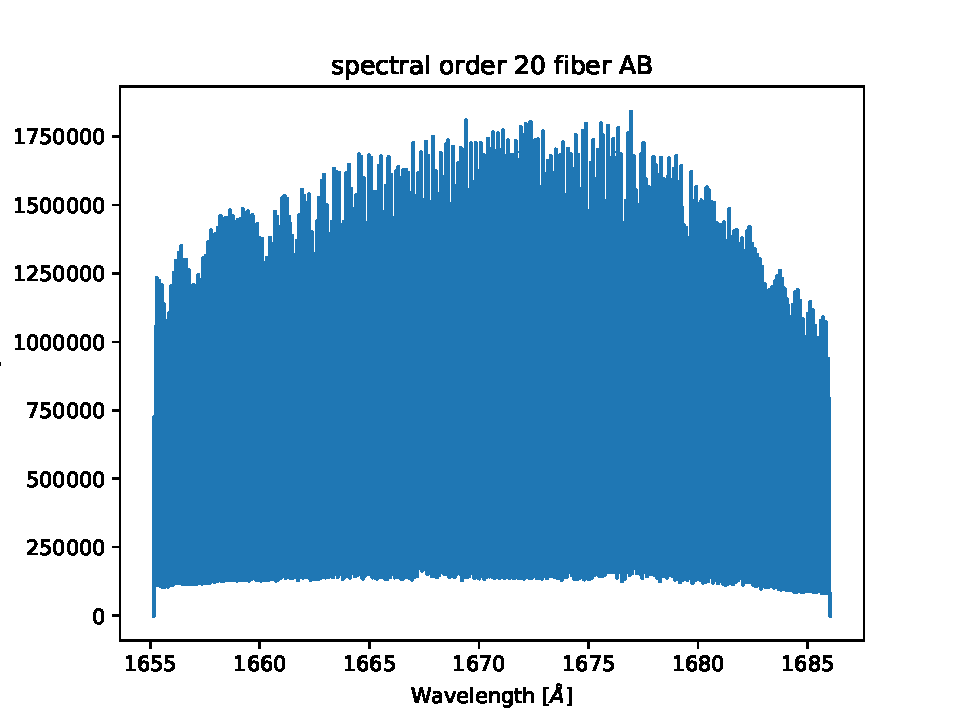
\includegraphics[width=\textwidth]{Figures/cal_ccf_e2ds_1.pdf}
a
\end{center}
\end{minipage}%
\begin{minipage}{.495\textwidth}
\begin{center}
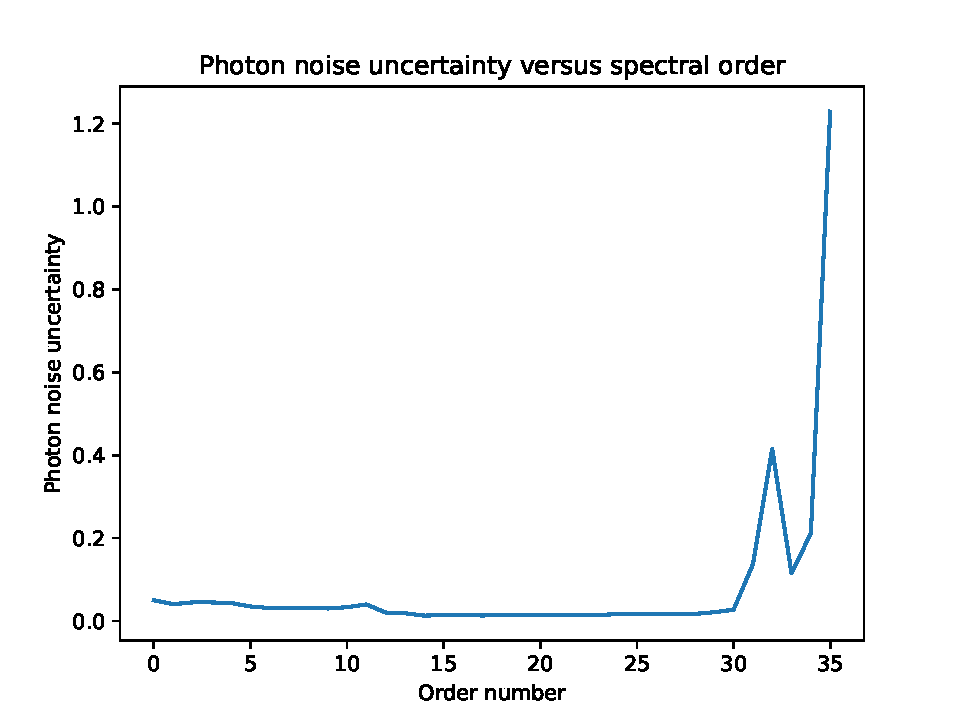
\includegraphics[width=\textwidth]{Figures/cal_ccf_e2ds_2.pdf}
b
\end{center}
\end{minipage}%
\end{center}

\begin{center}
\begin{minipage}{.495\textwidth}
\begin{center}
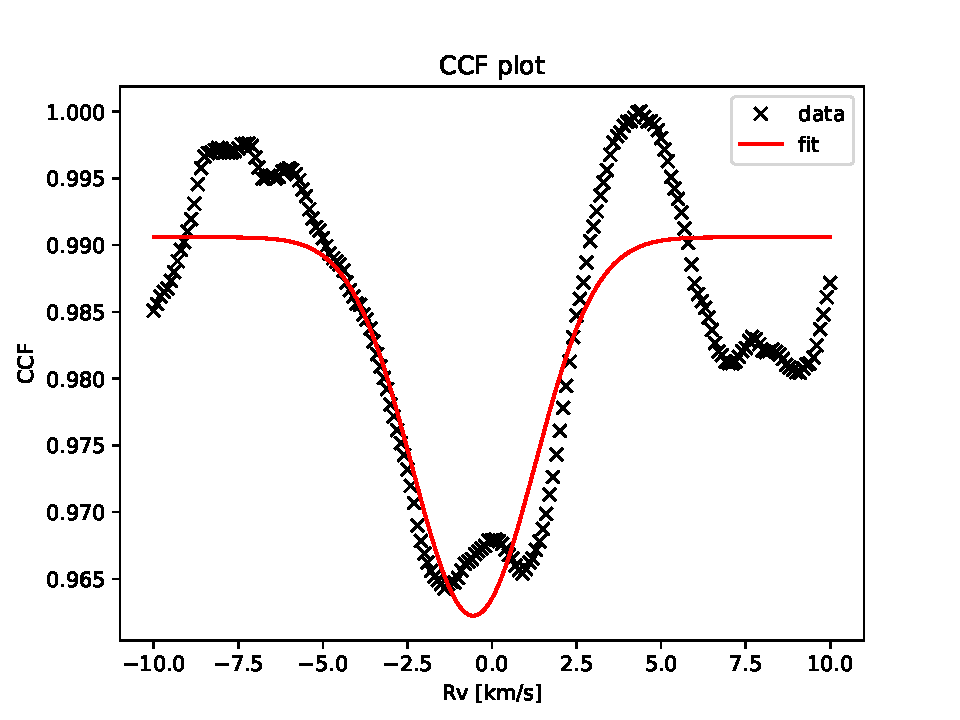
\includegraphics[width=\textwidth]{Figures/cal_ccf_e2ds_3.pdf}
c
\end{center}
\end{minipage}%
\end{center}

\caption{\textbf{(a)} The extract FP orders for spectral order 20, x-axis is wavelength and y-axis is extract flux. \textbf{(b)} Photon noise uncertainty versus spectral order. \textbf{(c)} The normalised CCF averaged across all orders, in red the fit to this CCF. \label{figure:cal_ccf_spirou}}
\end{figure}